\chapter{Teoretický základ}
\label{sec:te}
\begin{itemize}
    \item tcp/ip
    \item osi
    \item mqtt
    \item certifikát, k~tomu veřejný a soukromý klíč, self-signed jen treba lehce zminit, protoze je uz dost popsanej v~ty http sekci
    \item webové rozhraní
    \item relacni databaze, databazovy schema, vztahy (1:n, atd)
    \item navrhovy vzory -- mvc
\end{itemize}

\section{Názvosloví použité v~práci}

\begin{itemize}
    \item \textbf{Nadřazený systém} -- Zařízení, jehož tvorba je cílem práce, je v~textu označováno jako nadřazený systém. Podrobná specifikace nadřazeného systému je popsána v~úvodu kapitoly \ref{sec:an}.
    \item \textbf{Podřizený systém} -- Podřízené systémy jsou monitorovací zařízení, která jsou umístěná v~jednotlivých garážích. Zařízení neoperují samostatně, ale zasílají data nadřazenému systému. Podřízený systém je blíže popsán v~sekci \ref{sec:an_subsystem}.
    \item \textbf{Uživatel} -- uživatelem se v~textu práce myslí osoba spravující nadřazený systém a přistupující do jeho webového rozhraní. Jde tedy například o~majitele garáží nebo zaměstnance pověřeného jejich správou.
    \item \textbf{Klíč} -- Náhodně generovaná data (například ve formě textového řetězce), která slouží k~ověření totožnosti. Znalost klíče umožní přístup k~šifrovaným datům nebo jinak zakázaným operacím. V~této práci se hovoří většinou o~API klíčích, kterými se prokazují podřízené systémy při komunikaci s~nadřazeným systémem.
\end{itemize}

\section{Model \textit{client/server}}

\section{Model \textit{publisher/subscriber}}

\section{Protokol HTTP}

\subsection{Požadavek}
% u pozadavku popsat navratovy kod, metody, hlavicku

\subsection{Relace}

\subsection{HTTPS}

% \section{Cloud}

% \section{API} to mozna necham jen ve zkratkach, stejne tak JSON

% \section{Vícevláknová obsluha} ????

\section{CSRF -- \textit{Cross-site request forgery}}

CSRF je forma útoku na webovou aplikaci, při kterém může útočník odeslíat falešné požadavky pomocí prohlížeče přihlášeného uživatele \cite{csrf_owasp}. Útok může mít následující průběh:

\begin{enumerate}
    \item Uživatel je v~jedné záložce prohlížeče prihlášen do svého internetového bankovnictví, které není zabezpečeno proti CSRF.
    \item Útočník pošle uživateli odkaz na stránku, na který uživatel klikne.
    \item Stránka po načtení zašle požadavek internetovému bankovnictí, potvrzující převod peněz na útočníkův účet. Tento požadavek je platný, neboť pochází z~prohlížeče přihlášeného uživatele. Nezabezpečená aplikace internetového bankovnictví nemá jak ověřit, že požadavek nepřišel z~jejích stránek.
\end{enumerate}

Tento útok se dá použít k~zaslání nežádoucího požadavku (v~kontextu této práce například na smazání záznamu o~garáži), ne však ke získání dat ze stránky \cite{csrf_owasp}. Tomu zabraňuje koncept nazvaný \textit{same origin policy}, implementovaný v~současných prohlížečích \cite{sec_handbook}. Tento koncept omezuje to, jak spolu mohou interagovat webové stránky na různých doménách.

Ochranu proti CSRF je možné implementovat vkládáním náhodně generovaných \textit{tokenů} do formulářů na webové stránce. Při odeslání formuláře se pak původ požadavku ověří pomocí tohoto \textit{tokenu} -- zaslaný \textit{token} se musí shodovat s~\textit{tokenem} vloženým ve webové stránce.

Přihlášený uživatel má přístup k~webovým stránkam aplikace, a je tedy možné do odeslaného požadavku vložit ověřovací \textit{token} získaný z~formuláře. 

Naopak útočník může pouze zasílat požadavky, ale ne získávat data ze stránek, a tudíž nemá přístup k~\textit{tokenu}, kterým by mohl svůj požadavek zfalšovat.

Zde je opět důležitá \textit{same origin policy}, která získání \textit{tokenu} zabraňuje. Pokud by tento mechanismus nefungoval, mohl by útočník kromě zasílání požadavků také získávat data ze stránky, a tedy i platné \textit{tokeny}.

Webová aplikace implementovaná v~této práci využívá právě tento způsob ochrany proti CSRF (více v~sekci \ref{sec:im_controller}).

\section{\textit{Attack surface}}

\textit{Attack surface} popisuje všechny možné body, kde by mohl potencionální útočník napadnout daný systém \cite{attack_surface_owasp}. V~této práci je zmíněn v~sekci \ref{sec:an_cloud}, ve spojitosti se zvýšeným ohrožením při provozu serveru dostupného z~internetu.

\section{\textit{Man-in-the-middle} útok}

\textit{Man-in-the-middle} útok na protokolu HTTPS využívá situace, kdy certifikát pro ověření totožnosti serveru není důvěryhodný a může být zfalšován \cite{mitm}. 

V~tom případě může útočník (\textcolor{magenta}{Eva}) zachytit komunikaci mezi klientem (\textcolor{green}{Bob}) a serverem (\textcolor{blue2}{Alice}), a místo certifikátu serveru zaslat klientovi svůj certifikát. Poté je komunikace rozdělena na dvě části \cite{mitm}:

\begin{enumerate}
    \item \textcolor{green}{Bob} komunikuje s~\textcolor{magenta}{Evou} jako by to byla \textcolor{blue2}{Alice}. K~této komunikaci má \textcolor{magenta}{Eva} úplný přístup, neboť je šifrována pomocí jejího certifikátu.
    \item Po zachycení komunikace od \textcolor{green}{Boba} \textcolor{magenta}{Eva} tyto data přepošle \textcolor{blue2}{Alici}. \textcolor{blue2}{Alice} zašle \textcolor{magenta}{Evě} odpověď šifrovanou pomocí původního certifikátu. \textcolor{magenta}{Eva} tuto odpověď přečte, opět zašifruje pomocí svého certifikátu a pošle \textcolor{green}{Bobovi}.
\end{enumerate}

V~tomto scénáři \textcolor{green}{Bob} netuší, že nekomunikuje s~\textcolor{blue2}{Alicí}. Jelikož \textcolor{blue2}{Alice} nedodala důvěryhodný certifikát, nemůže \textcolor{green}{Bob} zjistit, že používá zfalšovaný.

\begin{figure}[h!]
    \centering
    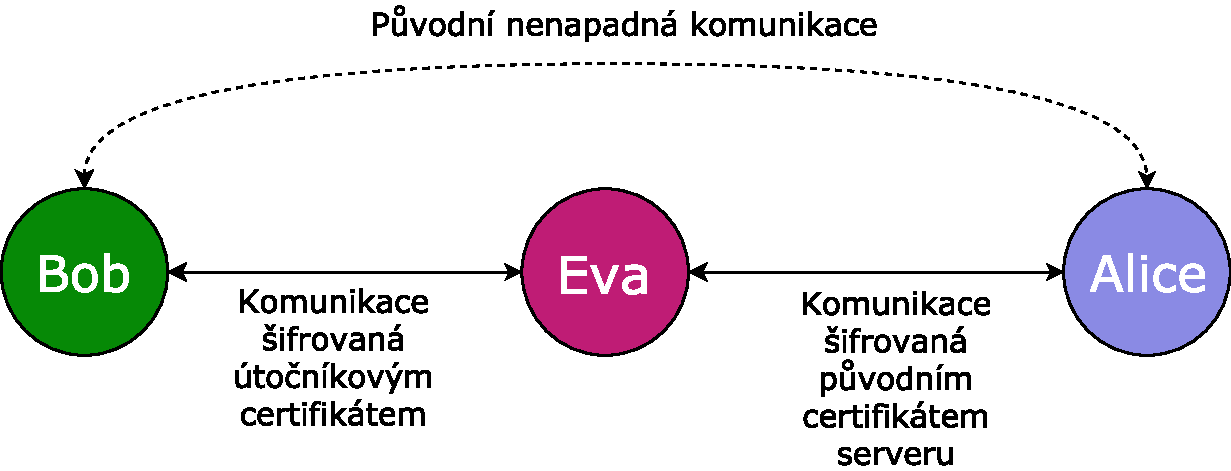
\includegraphics[width=\textwidth]{images/mitm.pdf}
    \caption[\textit{Man-in-the-middle} útok]{\textit{Man-in-the-middle} útok. Eva funguje jako nežádoucí prostředník mezi Bobem (klientem) a Alicí (původním serverem). Díky tomu má přístup ke zprávám obou účastníků komunikace. \cite{mitm}}
    \label{fig:mitm}
\end{figure}

V~textu práce je možnost \textit{man-in-the-middle} útoku diskutována v~části zabývající se volbou certifikátu pro provoz HTTPS (sekce \ref{sec:an_certs}).

\section{\textit{Hashování}}

\textit{Hashováním} se obecně rozumí vytvoření otistku pevné délky -- \textit{hashe} -- z~libovolných vstupních dat. Důležitou vlastností je jednosměrnost tohoto procesu, tedy že z~vytvořeného otisku již nelze (v~rozumném čase) zrekonstruovat původní vstup. \cite{hash_crackstation}

V~této práci je \textit{hashování} použito při ukládání hesel. Heslo uložené v~čitelné podobě není při úniku souboru s~heslem nijak chráněno. Proto je vhodné uložit místo hesla samotného jeho \textit{hash}. Pokud dojde k~úniku \textit{hashovaných} hesel, je pro útočníka velmi problematické získat z~otisků čitelná hesla \cite{hash_crackstation}.

\textit{Hashování} lze provést pomocí mnoha algortimů, ne všechny se však hodí k~zabezpečení ukládaných hesel. Některé algoritmy, jako například MD5 či SHA-1, nejsou dostatečně výpočetně náročné, takže umožňují efektivní útoky hrubou silou (lze dostatečně rychle spočítat všechny možné kombinace vstupů do dané délky a tím zjistit jaký vstup odpovídá danému \textit{hashi}) \cite{hash_crackstation}. 

Pro bezpečné ukládání hesel je tedy nutné použít dostatečné náročný algoritmus. V~této práci je použit algoritmus Argon2, který je považován za vhodný k~\textit{hashování} uložených hesel \cite{hash_crackstation}.

\subsection{Solení \textit{hashů}}

\textit{Hashování} hesla je vhodné doplnit o~proces takzvaného \uv{solení}. Při něm se nevytváří otisk samotného hesla, ale hesla doplněného o~náhodně vygenerovaný řetězec -- sůl. To ztěžuje použítí předpočítaných tabulek (například tabulky s~otisky často používaných hesel) pro útoky hrubou silou \cite{hash_crackstation}.

Pro bližší informace o~bezpečném ukládání hesel doporučuji článek \textit{Salted Password Hashing - Doing it Right} \cite{hash_crackstation}.
